\documentclass[12pt]{article}

\usepackage{orcidlink} % to insert a hyperlinked ORCiD logo
\usepackage{amssymb}
\usepackage{physics}
%\usepackage{cite} % may be useful for different formats of numerical citation
\usepackage{hyperref} % for hyperlinks in references

\usepackage{caption} % for \caption*

\textwidth 160mm
\textheight 230mm
\voffset = -20mm

\title{The article title}

\author{R.V.~Romanik, O.A.~Dobush,
	\\ \small Institute for Condensed Matter Physics, NAS of Ukraine 
	\\ \small 1~Svientsitskii Street, 79011, Lviv, Ukraine 
	\\ \small romanik@icmp.lviv.ua}
%\author{R.V.~Romanik \\ Institute for Condensed Matter Physics, NAS of Ukraine}

\begin{document}
	
	\maketitle
	
	%\begin{multicols}{2}
	
	\abstract{The topic of the article is studied in great details.
		\\	
		\textbf{Keywords:} Simple fluids, Critical behavior.
	}
	\section{Introduction}
	This topic has been very popular since the Large Hadron Collider (LHC) was built.
	
	For reference, see works~\cite{Cooper}
	
	\section{Thermal expansion coefficient}
	The dependence of the thermal expansion coefficient on density is shown in Fig.~\ref{fig4}
	
	\begin{figure}[h!]
		\centering 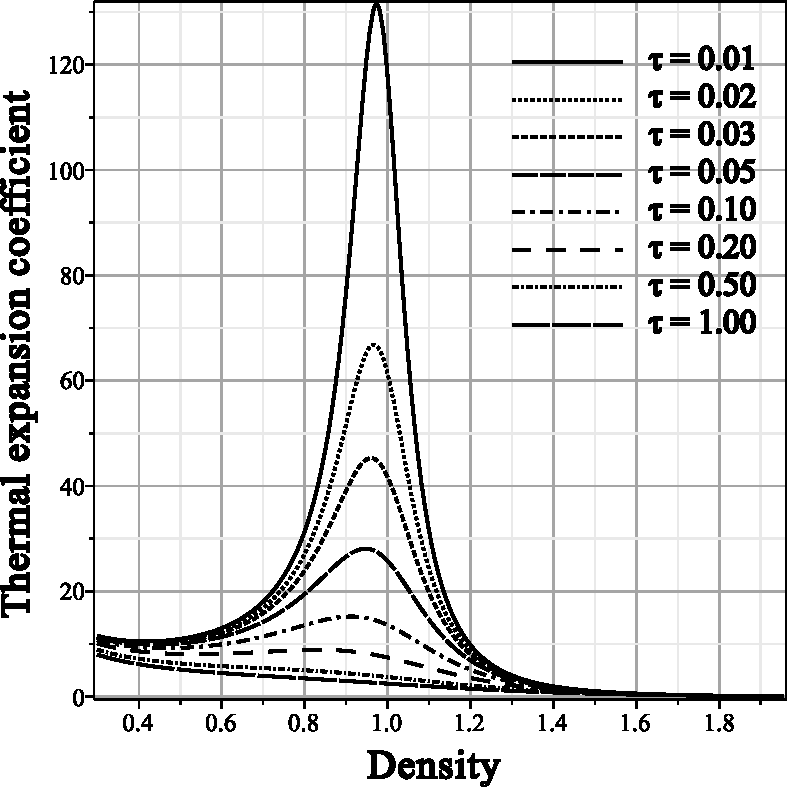
\includegraphics[width=0.5\textwidth]{f4.pdf}
		\vskip-3mm\caption{The thermal expansion coefficient $\alpha_P$ as a function of the density $\bar n$ at different values of reduced temperature $\tau > 0$ ($T > T_c$). 
		}\label{fig4}
	\end{figure}
	
	\section{Results and Discussion}
	Results go here. Discussion follows.
	
	\bibliographystyle{plain}
	\bibliography{Mbank}

\end{document}